\documentclass[12pt, twoside]{article}
\usepackage[letterpaper, margin=1in, headsep=0.5in]{geometry}
\usepackage[english]{babel}
\usepackage[utf8]{inputenc}
\usepackage{amsmath}
\usepackage{amsfonts}
\usepackage{amssymb}
\usepackage{tikz}
\usetikzlibrary{quotes, angles}
\usepackage{graphicx}
%\usepackage{pgfplots}
%\pgfplotsset{width=10cm,compat=1.9}
%\usepgfplotslibrary{statistics}
%\usepackage{pgfplotstable}
%\usepackage{tkz-fct}
%\usepackage{venndiagram}
\usepackage{enumitem}
\usepackage{multicol}


\usepackage{fancyhdr}
\pagestyle{fancy}
\fancyhf{}
\fancyhead[LE]{\thepage}
\fancyhead[RO]{%\thepage \\
    Name: \hspace{4cm} \,\\}
\fancyhead[LO]{BECA / Dr. Huson / Geometry 10th Grade\\* Unit 11: Algebra II introduction \\ 18 May 2020}

\renewcommand{\headrulewidth}{0pt}

\begin{document}
\subsubsection*{11.7 Problem set: Radian measures and standard trigonometry ratios}

\begin{enumerate}

  \item Two right triangles, $\triangle ABC$ and $\triangle ADE$, are shown in standard position with the coordinates of their vertices marked. \\[0.2cm]
  Identify each true statement. %\vspace{0.5cm}
  \begin{multicols}{2}
    \begin{enumerate}[itemsep=0.4cm]
      \item[$\square$ (a)] $AC=1$
      \item[$\square$ (b)] The altitude of $\triangle ADE$ is $\sqrt{3}$
      \item[$\square$ (c)] $\displaystyle \tan D= \frac{1}{\sqrt{3}}$
      \item[$\square$ (d)] $m\angle B = 60^\circ$
      \item[$\square$ (e)] $m\angle BAC = 60^\circ$
      \item[$\square$ (f)] $AD=2$
      \item[(g)] Explain why points $B$ and $D$ are on a circle centered at the origin. 
      \end{enumerate}
        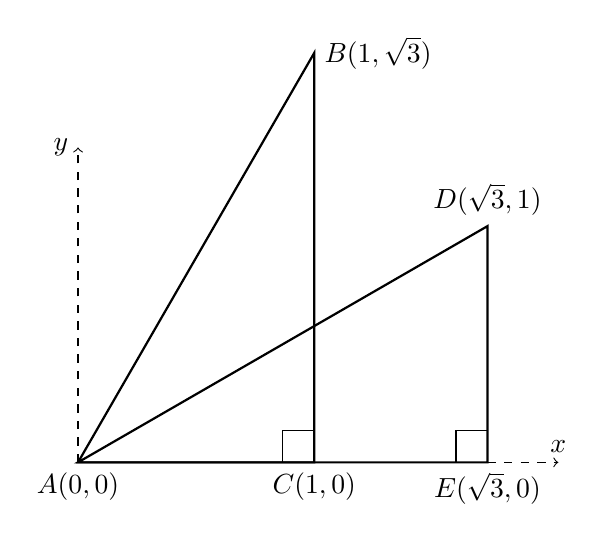
\begin{tikzpicture}[scale=1]
          \draw [dashed, ->] (5.2,0) -- (6.1,0) node [above] {$x$};
          \draw [dashed, ->] (0,0)--(0,4) node [left] {$y$};
          \draw [thick]
          (0,0)node[below]{$A(0,0)$}--
          (3,0)node[below]{$C(1,0)$}--
          (3,5.2)node[right]{$B(1,\sqrt{3})$}--cycle;
          \draw (3,0)++(-0.4,0)--++(0,0.4)--+(0.4,0);
          \draw [thick]
          (0,0)--(5.2,0)node[below]{$E(\sqrt{3},0)$}--
          (5.2,3)node[above]{$D(\sqrt{3},1)$}--cycle;
          \draw (5.2,0)++(-0.4,0)--++(0,0.4)--+(0.4,0);
          %\node at (1.5,0)[below]{$1$};
          %\node at (3,2.6)[right]{$\sqrt{3}$};
          %\node at (1.3,2.5)[above]{$2$};
        \end{tikzpicture}
    \end{multicols} \vspace{1.5cm}

    \item Simplify. Rationalize denominators.
    \begin{enumerate}
      \begin{multicols}{3}
        \item $\sqrt {27}$
        \item $\sqrt {18}+ 4\sqrt{3}$
        \item $\displaystyle \frac{3}{\sqrt{3}}$
      \end{multicols}
      \end{enumerate} \vspace{2cm}

  \item Convert the angle radian measure to degrees. (recall $360^\circ = 2\pi$ radians)
    \begin{enumerate}
      \begin{multicols}{3}
        \item $\displaystyle \frac{\pi}{6}$
        \item $\displaystyle \frac{\pi}{4}$
        \item $\displaystyle \frac{2\pi}{3}$
      \end{multicols}
      \end{enumerate} \vspace{1cm}
  
  \item Convert the degree measure to radians (state an \emph{exact} value, i.e. a fraction times $\pi$).
    \begin{enumerate}
      \begin{multicols}{3}
        \item $60^\circ$
        \item  $45^\circ$
        \item  $135^\circ$
      \end{multicols}
      \end{enumerate} %\vspace{4cm}

\end{enumerate}
\end{document}

